\documentclass[11pt,a4paper]{article}
\usepackage[margin=1in]{geometry}
\usepackage{graphicx}
\usepackage{hyperref}
\usepackage{booktabs}
\usepackage{float}
\usepackage{parskip}
\usepackage{enumitem}

\title{\textbf{Reproducing Figure 3 of LEXO:\\
LLM-Assisted Program Regeneration for Supply-Chain Security}}
\author{Abdelhak Chellal}
\date{May 2026}

\begin{document}

\maketitle

\section{Introduction}

This report documents my reproduction of Figure 3 from the paper
\textit{``Lexo: Eliminating Stealthy Supply-Chain Attacks via LLM-Assisted
Program Regeneration''} (Lamprou et al., 2025).

Modern software depends on thousands of third-party packages. Attackers can
inject malicious code that stays dormant until very specific conditions are
met — for example, activating only on a specific platform, only when a
certain environment variable is set, or only when connected to a live Bitcoin
network. These are called \textit{stealthy supply-chain attacks}. They evade
standard testing because the malicious behavior never triggers during normal
test runs.

LEXO's approach is simple: instead of trying to \textit{detect} malicious
code, it \textit{regenerates} the package from scratch using only observable
input/output behavior. Since malicious code causes side effects (network
calls, file access) rather than changing return values, it is invisible to the
regeneration process and does not appear in the new version.

Figure 3 of the paper evaluates regeneration correctness across 147 packages
and 4 LLM models. I reproduced this experiment on 13 packages and 7 models,
using simplifying assumptions where necessary.

\section{Methodology}

\subsection{The Pipeline}

I implemented the LEXO pipeline from scratch in Python, following the paper's
description and the exact prompts from Appendix A. The pipeline has three stages:

\begin{enumerate}[leftmargin=*]
  \item \textbf{Input generation.} An LLM reads the package source code and
  generates test inputs. For example, for \texttt{is-number}, the LLM generates
  inputs like \texttt{[42]}, \texttt{["hello"]}, \texttt{[null]}, \texttt{[true]}.

  \item \textbf{I/O pair collection.} Each input is run against the original
  package and the output is recorded — for example,
  \texttt{is-number(42) = true}, \texttt{is-number("hello") = false}. Malicious
  side effects are invisible here since only return values are captured.

  \item \textbf{Regeneration.} The LLM infers a natural language algorithm
  from the I/O pairs, then generates new clean code. The original source is
  never consulted again, severing any connection to malicious code.
\end{enumerate}

\subsection{Modifications to the Paper's Prompts}

The prompts from Appendix A were used as the base. Several additions were
necessary in practice:

\begin{itemize}[leftmargin=*]
  \item \textbf{Strict JSON rules.} LLMs frequently return non-JSON values
  (\texttt{NaN}, \texttt{undefined}, Python-style \texttt{True/False}) or add
  comments inside JSON. A \texttt{STRICT RULES} block was added explicitly
  forbidding these.

  \item \textbf{Input format change.} The paper uses JavaScript expression
  syntax (e.g. \texttt{[x => x + 1]}) which Python cannot parse. We use JSON
  arrays of arrays (\texttt{[[1], [0], [-1]]}). The goal is identical — the
  LLM suggests inputs, the system runs them to get real outputs.

  \item \textbf{Function argument serialization.} \texttt{concat-map} and
  \texttt{just-filter-object} take functions as arguments, which are not
  JSON-serializable. These are serialized as strings and \texttt{eval()}'d at
  runtime: \texttt{[[1,2,3], "function(x)\{ return x*2; \}"]}.

  \item \textbf{Retry with stricter reminder.} On failure, the model is retried
  up to 3 times with a stronger JSON format reminder and lower temperature
  (0.3 vs 0.7). The paper uses a coverage-guided revision loop; we use a
  simpler JSON-parse-failure trigger.
\end{itemize}

\subsection{Models}

The paper uses GPT-5 mini, GPT-4o, GPT-3.5, and Mistral 7B. I made the
following changes:

\begin{itemize}[leftmargin=*]
  \item \textbf{GPT-5 mini} was substituted with \textbf{GPT-5.4 mini} —
  the original ID (\texttt{openai/gpt-5-mini}) returned empty responses via
  OpenRouter.
  \item \textbf{GPT-4o} was substituted with \textbf{GPT-4o mini} due to
  cost.
  \item Three models were added beyond the paper's set: \textbf{Claude 3.5
  Haiku}, \textbf{DeepSeek V4 Flash}, and \textbf{Owl Alpha}, to extend the
  comparison.
\end{itemize}

All models were accessed via OpenRouter at a total cost under \$1 for all
experiments.

\subsection{Packages}

I evaluated 13 of the 15 packages from Table 2 of the paper. Two were dropped:
\texttt{fast\_blank} (Ruby C extension — bundler version conflicts) and
\texttt{character-count} (C++ NAN library incompatible with Node.js v20).
A third, \texttt{split-on-first}, was dropped due to ESM/CommonJS
incompatibility. These represent infrastructure limitations unrelated to the
LEXO pipeline itself.

For \texttt{primality} (Python), I regenerated 6 of 7 functions. The 7th
(\texttt{rand\_prime}) was added as a simple wrapper around \texttt{between()}
with \texttt{random.choice()}.

\section{Results}

\begin{table}[H]
\centering
\begin{tabular}{lrrr}
\toprule
\textbf{Model} & \textbf{Paper equiv.} & \textbf{At 100\%} & \textbf{Avg score} \\
\midrule
GPT-5.4 mini      & GPT-5 mini  & 9/13 & 80.1\% \\
Owl Alpha          & —           & 4/13 & 52.0\% \\
DeepSeek V4 Flash  & —           & 5/13 & 49.5\% \\
GPT-4o mini        & GPT-4o      & 2/13 & 41.3\% \\
Claude 3.5 Haiku   & —           & 3/13 & 38.7\% \\
GPT-3.5 Turbo      & GPT-3.5     & 1/13 & 32.2\% \\
Mistral 7B         & Mistral 7B  & 0/13 & 11.9\% \\
\bottomrule
\end{tabular}
\caption{Final results (3 retries, 13 packages). ``At 100\%'' = passed all
developer tests.}
\end{table}

\begin{figure}[H]
  \centering
  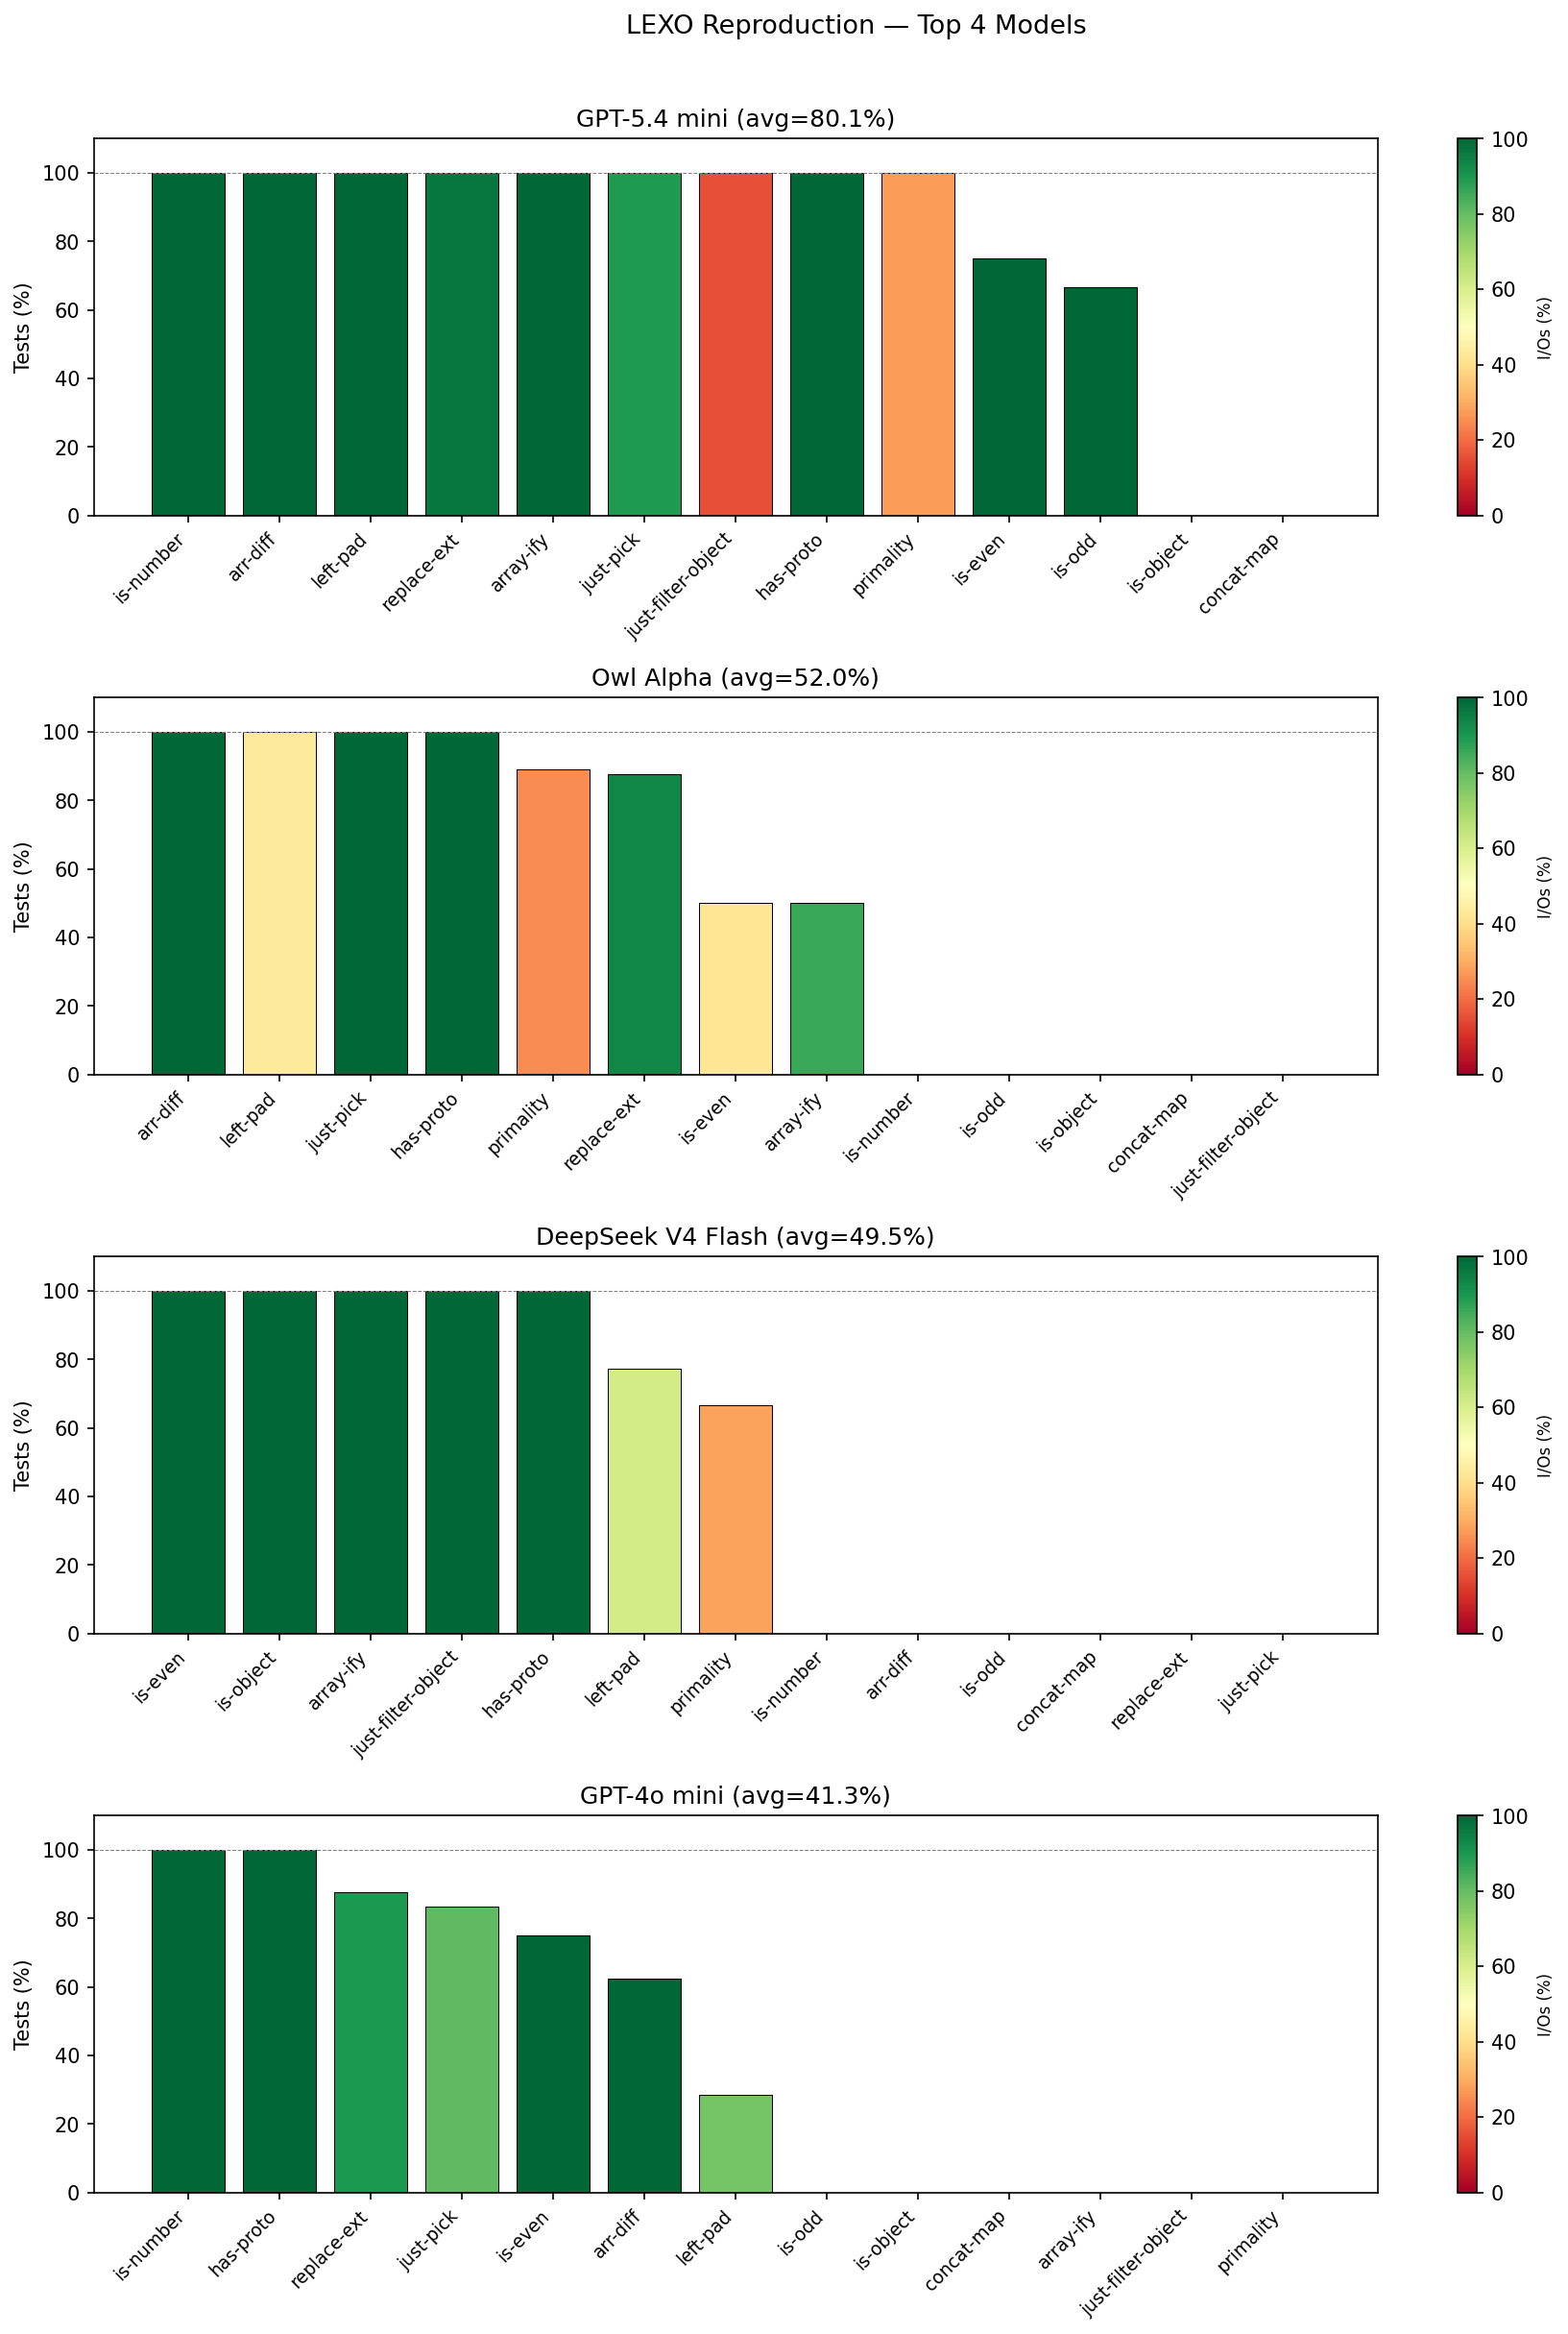
\includegraphics[width=\textwidth]{results/figure3_top4.png}
  \caption{Top 4 models by average score. Each bar = one package. Bar height
  = \% of developer tests passed. Color = \% of I/O pairs matched
  (dark green = high, red = low).}
\end{figure}

\begin{figure}[H]
  \centering
  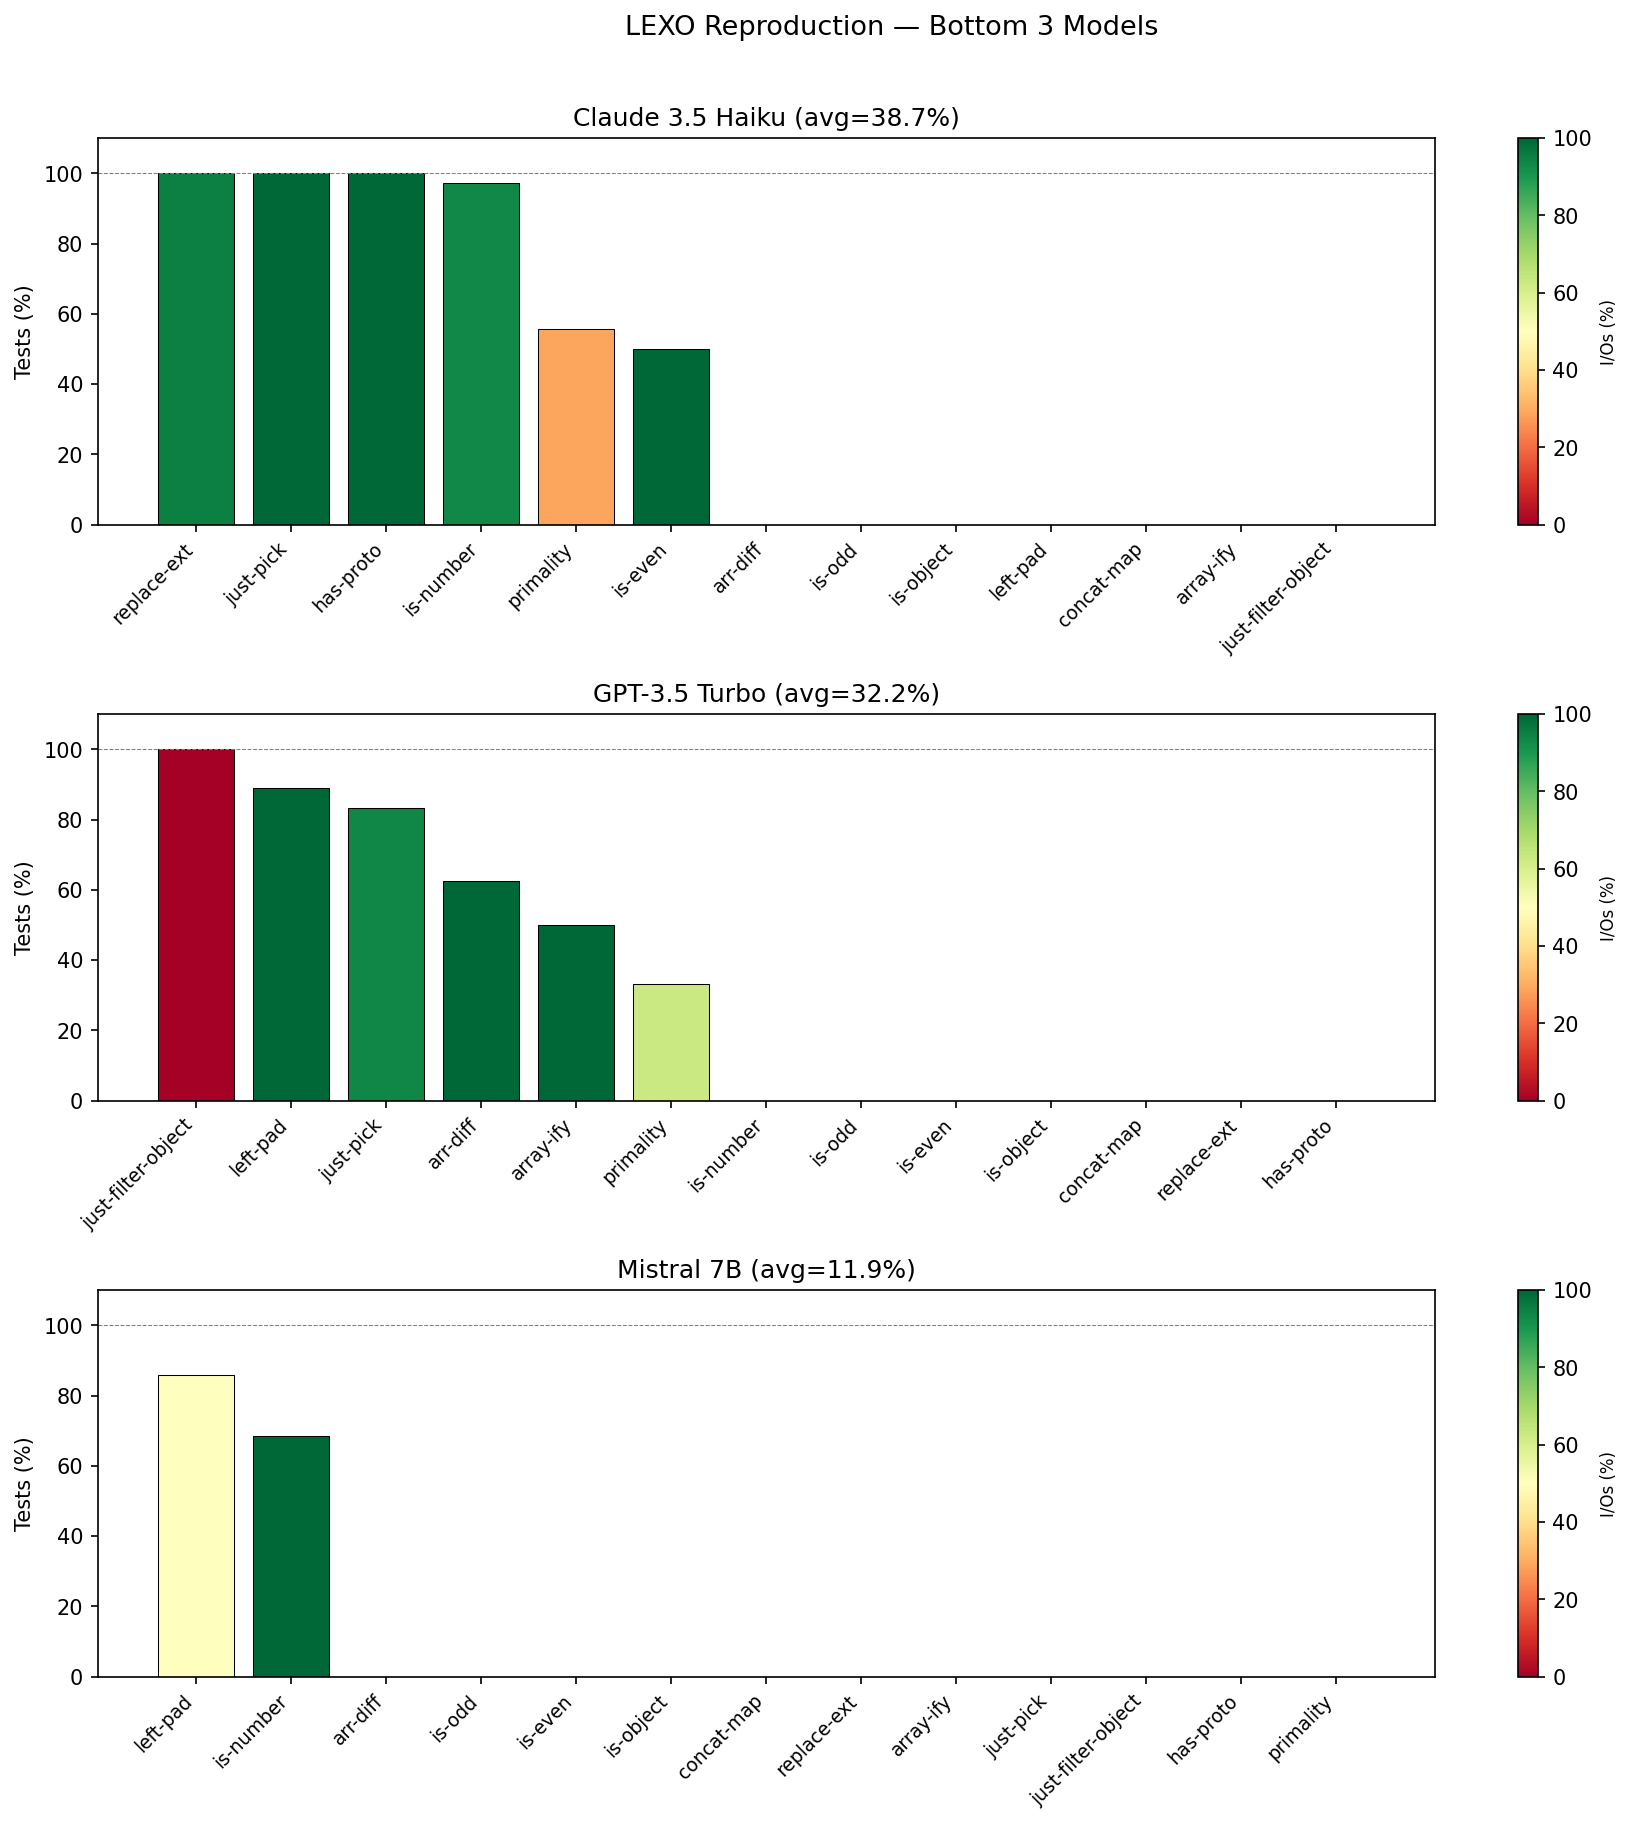
\includegraphics[width=\textwidth]{results/figure3_bottom3.png}
  \caption{Bottom 3 models. Same axes.}
\end{figure}

\subsection{Comparison with the Paper}

\begin{table}[H]
\centering
\begin{tabular}{lrr}
\toprule
\textbf{Model} & \textbf{Paper (147 pkgs, at 100\%)} & \textbf{Ours (13 pkgs, at 100\%)} \\
\midrule
GPT-5 mini / GPT-5.4 mini & 86/147 (59\%) & 9/13 (69\%) \\
GPT-4o / GPT-4o mini       & 59/147 (40\%) & 2/13 (15\%) \\
GPT-3.5 Turbo              & 35/147 (24\%) & 1/13 (8\%)  \\
Mistral 7B                 & 3/147 (2\%)   & 0/13 (0\%)  \\
\bottomrule
\end{tabular}
\caption{Comparison with paper results.}
\end{table}

The ordering of models matches the paper exactly: GPT-5 mini $>$ GPT-4o $>$
GPT-3.5 $>$ Mistral 7B. Our percentages for GPT-4o mini and GPT-3.5 are lower
than the paper's, which is expected — the paper implements a full
coverage-guided revision loop that we did not replicate, and evaluates more
packages reducing the variance.

\section{Observations}

\textbf{The idea is simple and powerful.} LEXO does not need to understand
malicious code at all. The key insight — that malicious behavior is
side-effectful and therefore invisible in return values — makes the approach
elegant and robust. I find it a great example of solving a hard problem by
reframing it.

\textbf{LLM non-determinism is a real challenge.} The same prompt, same
package, and same model can succeed on one run and fail with a JSON parse error
on the next. Building a reliable pipeline on top of non-deterministic models
requires significant engineering effort — retry logic, output normalization, and
format enforcement. The paper acknowledges this with its revision loop, but even
so, perfect reliability is not guaranteed.

\textbf{Model quality is the bottleneck.} Most failures were not code
generation failures — they were input generation failures. Weaker models
(Mistral, GPT-3.5) could not reliably produce valid JSON even after 3 retries.
This points to an interesting research direction: fine-tuning small open-source
models specifically on structured JSON output tasks could make LEXO viable
without expensive frontier models.

\textbf{The cost is negligible.} All experiments — multiple runs across 7
models and 13 packages — cost under \$1. This makes LEXO practical for real
CI/CD pipelines.

\textbf{Language-agnostic in theory, engineering-intensive in practice.} The
paper claims LEXO is language-agnostic, which is conceptually true. In practice,
each language requires custom serialization, test framework parsing, and runtime
integration. Ruby and C++ packages could not be included due to native
compilation failures, and Python required a separate sub-pipeline.

\section{Conclusion}

This reproduction confirms the paper's core finding: stronger LLMs produce
better regenerations, and the approach is practical and cheap. The model
ordering in our results matches the paper exactly.

The main gap is the absence of a coverage-guided revision loop, which the
paper shows is important for correctness. Implementing it fully, and exploring
whether fine-tuned smaller models could replace frontier models for this task,
would be interesting directions for future work.

\bigskip
\noindent\textbf{Repository:} \url{https://github.com/Abdelhak-Chellal/Lexo-repro}\\
\noindent\textbf{Total API cost:} $<$ \$1 across all experiments.

\end{document}